\documentclass[twoside]{book}

% Packages required by doxygen
\usepackage{fixltx2e}
\usepackage{calc}
\usepackage{doxygen}
\usepackage[export]{adjustbox} % also loads graphicx
\usepackage{graphicx}
\usepackage[utf8]{inputenc}
\usepackage{makeidx}
\usepackage{multicol}
\usepackage{multirow}
\PassOptionsToPackage{warn}{textcomp}
\usepackage{textcomp}
\usepackage[nointegrals]{wasysym}
\usepackage[table]{xcolor}

% Font selection
\usepackage[T1]{fontenc}
\usepackage[scaled=.90]{helvet}
\usepackage{courier}
\usepackage{amssymb}
\usepackage{sectsty}
\renewcommand{\familydefault}{\sfdefault}
\allsectionsfont{%
  \fontseries{bc}\selectfont%
  \color{darkgray}%
}
\renewcommand{\DoxyLabelFont}{%
  \fontseries{bc}\selectfont%
  \color{darkgray}%
}
\newcommand{\+}{\discretionary{\mbox{\scriptsize$\hookleftarrow$}}{}{}}

% Page & text layout
\usepackage{geometry}
\geometry{%
  a4paper,%
  top=2.5cm,%
  bottom=2.5cm,%
  left=2.5cm,%
  right=2.5cm%
}
\tolerance=750
\hfuzz=15pt
\hbadness=750
\setlength{\emergencystretch}{15pt}
\setlength{\parindent}{0cm}
\setlength{\parskip}{3ex plus 2ex minus 2ex}
\makeatletter
\renewcommand{\paragraph}{%
  \@startsection{paragraph}{4}{0ex}{-1.0ex}{1.0ex}{%
    \normalfont\normalsize\bfseries\SS@parafont%
  }%
}
\renewcommand{\subparagraph}{%
  \@startsection{subparagraph}{5}{0ex}{-1.0ex}{1.0ex}{%
    \normalfont\normalsize\bfseries\SS@subparafont%
  }%
}
\makeatother

% Headers & footers
\usepackage{fancyhdr}
\pagestyle{fancyplain}
\fancyhead[LE]{\fancyplain{}{\bfseries\thepage}}
\fancyhead[CE]{\fancyplain{}{}}
\fancyhead[RE]{\fancyplain{}{\bfseries\leftmark}}
\fancyhead[LO]{\fancyplain{}{\bfseries\rightmark}}
\fancyhead[CO]{\fancyplain{}{}}
\fancyhead[RO]{\fancyplain{}{\bfseries\thepage}}
\fancyfoot[LE]{\fancyplain{}{}}
\fancyfoot[CE]{\fancyplain{}{}}
\fancyfoot[RE]{\fancyplain{}{\bfseries\scriptsize Generated by Doxygen }}
\fancyfoot[LO]{\fancyplain{}{\bfseries\scriptsize Generated by Doxygen }}
\fancyfoot[CO]{\fancyplain{}{}}
\fancyfoot[RO]{\fancyplain{}{}}
\renewcommand{\footrulewidth}{0.4pt}
\renewcommand{\chaptermark}[1]{%
  \markboth{#1}{}%
}
\renewcommand{\sectionmark}[1]{%
  \markright{\thesection\ #1}%
}

% Indices & bibliography
\usepackage{natbib}
\usepackage[titles]{tocloft}
\setcounter{tocdepth}{3}
\setcounter{secnumdepth}{5}
\makeindex

% Hyperlinks (required, but should be loaded last)
\usepackage{ifpdf}
\ifpdf
  \usepackage[pdftex,pagebackref=true]{hyperref}
\else
  \usepackage[ps2pdf,pagebackref=true]{hyperref}
\fi
\hypersetup{%
  colorlinks=true,%
  linkcolor=blue,%
  citecolor=blue,%
  unicode%
}

% Custom commands
\newcommand{\clearemptydoublepage}{%
  \newpage{\pagestyle{empty}\cleardoublepage}%
}

\usepackage{caption}
\captionsetup{labelsep=space,justification=centering,font={bf},singlelinecheck=off,skip=4pt,position=top}

%===== C O N T E N T S =====

\begin{document}

% Titlepage & ToC
\hypersetup{pageanchor=false,
             bookmarksnumbered=true,
             pdfencoding=unicode
            }
\pagenumbering{alph}
\begin{titlepage}
\vspace*{7cm}
\begin{center}%
{\Large Coulomb Solver }\\
\vspace*{1cm}
{\large Generated by Doxygen 1.8.13}\\
\end{center}
\end{titlepage}
\clearemptydoublepage
\pagenumbering{roman}
\tableofcontents
\clearemptydoublepage
\pagenumbering{arabic}
\hypersetup{pageanchor=true}

%--- Begin generated contents ---
\chapter{Hierarchical Index}
\section{Class Hierarchy}
This inheritance list is sorted roughly, but not completely, alphabetically\+:\begin{DoxyCompactList}
\item Base\begin{DoxyCompactList}
\item \contentsline{section}{Binary\+Op$<$ Expr1, Expr2, operation $>$}{\pageref{structBinaryOp}}{}
\end{DoxyCompactList}
\item \contentsline{section}{Chunk}{\pageref{structChunk}}{}
\item \contentsline{section}{Coulomb\+Solver}{\pageref{classCoulombSolver}}{}
\item \contentsline{section}{Expr\+Size$<$ Expr $>$}{\pageref{classExprSize}}{}
\item \contentsline{section}{Expr\+Size$<$ Expr1 $>$}{\pageref{classExprSize}}{}
\begin{DoxyCompactList}
\item \contentsline{section}{Expr\+Size$<$ Binary\+Op$<$ Expr1, Expr2, operation $>$ $>$}{\pageref{classExprSize_3_01BinaryOp_3_01Expr1_00_01Expr2_00_01operation_01_4_01_4}}{}
\end{DoxyCompactList}
\item integral\+\_\+constant\begin{DoxyCompactList}
\item \contentsline{section}{Expr\+Size$<$ Vector$<$ T, n $>$ $>$}{\pageref{classExprSize_3_01Vector_3_01T_00_01n_01_4_01_4}}{}
\end{DoxyCompactList}
\item \contentsline{section}{Memory\+Mapped\+File}{\pageref{classMemoryMappedFile}}{}
\item \contentsline{section}{parse\+Chunk}{\pageref{structparseChunk}}{}
\item \contentsline{section}{Vector$<$ T, n $>$}{\pageref{structVector}}{}
\end{DoxyCompactList}

\chapter{Class Index}
\section{Class List}
Here are the classes, structs, unions and interfaces with brief descriptions\+:\begin{DoxyCompactList}
\item\contentsline{section}{\hyperlink{structBinaryOp}{Binary\+Op$<$ Expr1, Expr2, operation $>$} }{\pageref{structBinaryOp}}{}
\item\contentsline{section}{\hyperlink{structChunk}{Chunk} }{\pageref{structChunk}}{}
\item\contentsline{section}{\hyperlink{classCoulombSolver}{Coulomb\+Solver} \\*Class to perform a single time step to solve the coulomb equation }{\pageref{classCoulombSolver}}{}
\item\contentsline{section}{\hyperlink{classExprSize}{Expr\+Size$<$ Expr $>$} }{\pageref{classExprSize}}{}
\item\contentsline{section}{\hyperlink{classExprSize_3_01BinaryOp_3_01Expr1_00_01Expr2_00_01operation_01_4_01_4}{Expr\+Size$<$ Binary\+Op$<$ Expr1, Expr2, operation $>$ $>$} }{\pageref{classExprSize_3_01BinaryOp_3_01Expr1_00_01Expr2_00_01operation_01_4_01_4}}{}
\item\contentsline{section}{\hyperlink{classExprSize_3_01Vector_3_01T_00_01n_01_4_01_4}{Expr\+Size$<$ Vector$<$ T, n $>$ $>$} }{\pageref{classExprSize_3_01Vector_3_01T_00_01n_01_4_01_4}}{}
\item\contentsline{section}{\hyperlink{classMemoryMappedFile}{Memory\+Mapped\+File} }{\pageref{classMemoryMappedFile}}{}
\item\contentsline{section}{\hyperlink{structparseChunk}{parse\+Chunk} }{\pageref{structparseChunk}}{}
\item\contentsline{section}{\hyperlink{structVector}{Vector$<$ T, n $>$} }{\pageref{structVector}}{}
\end{DoxyCompactList}

\chapter{Class Documentation}
\hypertarget{structBinaryOp}{}\section{Binary\+Op$<$ Expr1, Expr2, operation $>$ Struct Template Reference}
\label{structBinaryOp}\index{Binary\+Op$<$ Expr1, Expr2, operation $>$@{Binary\+Op$<$ Expr1, Expr2, operation $>$}}


Inheritance diagram for Binary\+Op$<$ Expr1, Expr2, operation $>$\+:
\nopagebreak
\begin{figure}[H]
\begin{center}
\leavevmode
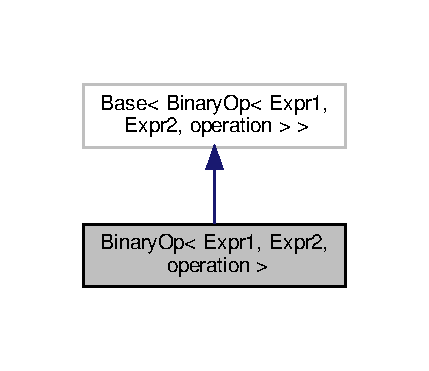
\includegraphics[width=206pt]{structBinaryOp__inherit__graph}
\end{center}
\end{figure}


Collaboration diagram for Binary\+Op$<$ Expr1, Expr2, operation $>$\+:
\nopagebreak
\begin{figure}[H]
\begin{center}
\leavevmode
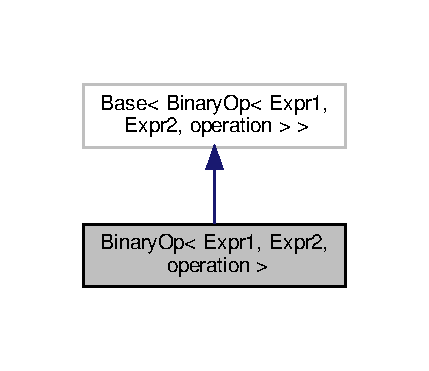
\includegraphics[width=206pt]{structBinaryOp__coll__graph}
\end{center}
\end{figure}
\subsection*{Public Types}
\begin{DoxyCompactItemize}
\item 
\mbox{\Hypertarget{structBinaryOp_aa0a5ecc4e1659195bf8c46f70f52adf0}\label{structBinaryOp_aa0a5ecc4e1659195bf8c46f70f52adf0}} 
using {\bfseries Scalar} = typename Expr1\+::\+Scalar
\end{DoxyCompactItemize}
\subsection*{Public Member Functions}
\begin{DoxyCompactItemize}
\item 
\mbox{\Hypertarget{structBinaryOp_abe24eb2101260539e40e079163658c18}\label{structBinaryOp_abe24eb2101260539e40e079163658c18}} 
constexpr Scalar \& {\bfseries operator\mbox{[}$\,$\mbox{]}} (const int index)
\end{DoxyCompactItemize}
\subsection*{Public Attributes}
\begin{DoxyCompactItemize}
\item 
\mbox{\Hypertarget{structBinaryOp_a149d1150d0ddde47299bcf55a79b17bd}\label{structBinaryOp_a149d1150d0ddde47299bcf55a79b17bd}} 
const Expr1 \& {\bfseries expr1}
\item 
\mbox{\Hypertarget{structBinaryOp_a2719a5e3c601f4048019b34cb011c6c1}\label{structBinaryOp_a2719a5e3c601f4048019b34cb011c6c1}} 
const Expr2 \& {\bfseries expr2}
\end{DoxyCompactItemize}


The documentation for this struct was generated from the following file\+:\begin{DoxyCompactItemize}
\item 
src/binary\+\_\+operations.\+hpp\end{DoxyCompactItemize}

\hypertarget{structChunk}{}\section{Chunk Struct Reference}
\label{structChunk}\index{Chunk@{Chunk}}
\subsection*{Public Member Functions}
\begin{DoxyCompactItemize}
\item 
\mbox{\Hypertarget{structChunk_a6bcebb0e47d7edcdfc0814efd2aef1ae}\label{structChunk_a6bcebb0e47d7edcdfc0814efd2aef1ae}} 
{\bfseries Chunk} (const char $\ast$begin, const char $\ast$new\+Line)
\end{DoxyCompactItemize}
\subsection*{Public Attributes}
\begin{DoxyCompactItemize}
\item 
\mbox{\Hypertarget{structChunk_ac1330b0d79577428a3727b8a383c53c3}\label{structChunk_ac1330b0d79577428a3727b8a383c53c3}} 
const char $\ast$ {\bfseries begin}
\item 
\mbox{\Hypertarget{structChunk_a17555e7645ce9415de721cc682d18346}\label{structChunk_a17555e7645ce9415de721cc682d18346}} 
const char $\ast$ {\bfseries new\+Line}
\end{DoxyCompactItemize}


The documentation for this struct was generated from the following file\+:\begin{DoxyCompactItemize}
\item 
src/file\+\_\+io.\+cpp\end{DoxyCompactItemize}

\hypertarget{classCoulombSolver}{}\section{Coulomb\+Solver Class Reference}
\label{classCoulombSolver}\index{Coulomb\+Solver@{Coulomb\+Solver}}


Class to perform a single time step to solve the coulomb equation.  




{\ttfamily \#include $<$coulomb\+\_\+solver.\+hpp$>$}

\subsection*{Public Member Functions}
\begin{DoxyCompactItemize}
\item 
void \hyperlink{classCoulombSolver_ad336b4a87ab865aa75dd86860862aa81}{set\+Charges} (const std\+::vector$<$ \hyperlink{structVector}{Vector4f} $>$ $\ast$charges)
\item 
{\footnotesize template$<$bool Compute\+Potentials$>$ }\\std\+::vector$<$ \hyperlink{structVector}{Vector4f} $>$ \hyperlink{classCoulombSolver_a5a0cbb3931a1b1939673b9ee918a4300}{solve} ()
\end{DoxyCompactItemize}


\subsection{Detailed Description}
Class to perform a single time step to solve the coulomb equation. 

Detailed description follows here. \begin{DoxyAuthor}{Author}
Janos Meny 
\end{DoxyAuthor}
\begin{DoxyDate}{Date}
August 2019 
\end{DoxyDate}


\subsection{Member Function Documentation}
\mbox{\Hypertarget{classCoulombSolver_ad336b4a87ab865aa75dd86860862aa81}\label{classCoulombSolver_ad336b4a87ab865aa75dd86860862aa81}} 
\index{Coulomb\+Solver@{Coulomb\+Solver}!set\+Charges@{set\+Charges}}
\index{set\+Charges@{set\+Charges}!Coulomb\+Solver@{Coulomb\+Solver}}
\subsubsection{\texorpdfstring{set\+Charges()}{setCharges()}}
{\footnotesize\ttfamily void Coulomb\+Solver\+::set\+Charges (\begin{DoxyParamCaption}\item[{const std\+::vector$<$ \hyperlink{structVector}{Vector4f} $>$ $\ast$}]{charges }\end{DoxyParamCaption})}

Setter function for particles. The first three components of each Vector3f describe the x, y and z component, the 4\textquotesingle{}th component stores the charge q. 
\begin{DoxyParams}{Parameters}
{\em charges} & -\/ particles and charges \\
\hline
\end{DoxyParams}
\begin{DoxyReturn}{Returns}
void 
\end{DoxyReturn}
\mbox{\Hypertarget{classCoulombSolver_a5a0cbb3931a1b1939673b9ee918a4300}\label{classCoulombSolver_a5a0cbb3931a1b1939673b9ee918a4300}} 
\index{Coulomb\+Solver@{Coulomb\+Solver}!solve@{solve}}
\index{solve@{solve}!Coulomb\+Solver@{Coulomb\+Solver}}
\subsubsection{\texorpdfstring{solve()}{solve()}}
{\footnotesize\ttfamily template$<$bool Compute\+Potentials$>$ \\
std\+::vector$<$ \hyperlink{structVector}{Vector4f} $>$ Coulomb\+Solver\+::solve (\begin{DoxyParamCaption}{ }\end{DoxyParamCaption})}

Solves one time step of the coulomb equation. 
\begin{DoxyParams}{Parameters}
{\em bool} & -\/ Compute\+Potentials, if this is true, in the the forth component will contain also the force potentials. \\
\hline
\end{DoxyParams}
\begin{DoxyReturn}{Returns}
a vector of Vector4f 
\end{DoxyReturn}


The documentation for this class was generated from the following files\+:\begin{DoxyCompactItemize}
\item 
src/coulomb\+\_\+solver.\+hpp\item 
src/coulomb\+\_\+solver.\+cpp\end{DoxyCompactItemize}

\hypertarget{classExprSize}{}\section{Expr\+Size$<$ Expr $>$ Class Template Reference}
\label{classExprSize}\index{Expr\+Size$<$ Expr $>$@{Expr\+Size$<$ Expr $>$}}


The documentation for this class was generated from the following file\+:\begin{DoxyCompactItemize}
\item 
src/vector\+\_\+traits.\+hpp\end{DoxyCompactItemize}

\hypertarget{classExprSize_3_01BinaryOp_3_01Expr1_00_01Expr2_00_01operation_01_4_01_4}{}\section{Expr\+Size$<$ Binary\+Op$<$ Expr1, Expr2, operation $>$ $>$ Class Template Reference}
\label{classExprSize_3_01BinaryOp_3_01Expr1_00_01Expr2_00_01operation_01_4_01_4}\index{Expr\+Size$<$ Binary\+Op$<$ Expr1, Expr2, operation $>$ $>$@{Expr\+Size$<$ Binary\+Op$<$ Expr1, Expr2, operation $>$ $>$}}


Inheritance diagram for Expr\+Size$<$ Binary\+Op$<$ Expr1, Expr2, operation $>$ $>$\+:
\nopagebreak
\begin{figure}[H]
\begin{center}
\leavevmode
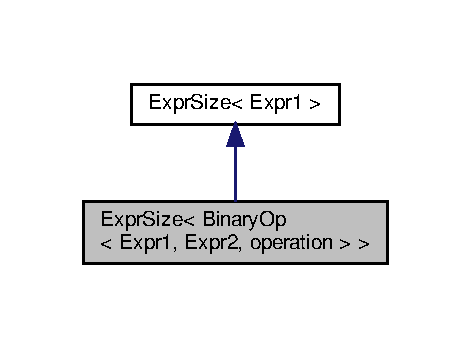
\includegraphics[width=226pt]{classExprSize_3_01BinaryOp_3_01Expr1_00_01Expr2_00_01operation_01_4_01_4__inherit__graph}
\end{center}
\end{figure}


Collaboration diagram for Expr\+Size$<$ Binary\+Op$<$ Expr1, Expr2, operation $>$ $>$\+:
\nopagebreak
\begin{figure}[H]
\begin{center}
\leavevmode
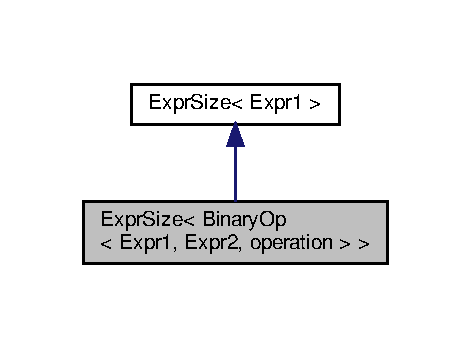
\includegraphics[width=226pt]{classExprSize_3_01BinaryOp_3_01Expr1_00_01Expr2_00_01operation_01_4_01_4__coll__graph}
\end{center}
\end{figure}


The documentation for this class was generated from the following file\+:\begin{DoxyCompactItemize}
\item 
src/vector\+\_\+traits.\+hpp\end{DoxyCompactItemize}

\hypertarget{classExprSize_3_01Vector_3_01T_00_01n_01_4_01_4}{}\section{Expr\+Size$<$ Vector$<$ T, n $>$ $>$ Class Template Reference}
\label{classExprSize_3_01Vector_3_01T_00_01n_01_4_01_4}\index{Expr\+Size$<$ Vector$<$ T, n $>$ $>$@{Expr\+Size$<$ Vector$<$ T, n $>$ $>$}}


Inheritance diagram for Expr\+Size$<$ Vector$<$ T, n $>$ $>$\+:
\nopagebreak
\begin{figure}[H]
\begin{center}
\leavevmode
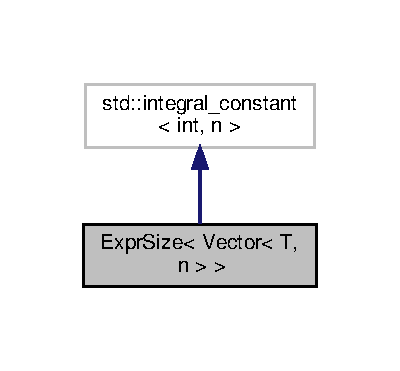
\includegraphics[width=192pt]{classExprSize_3_01Vector_3_01T_00_01n_01_4_01_4__inherit__graph}
\end{center}
\end{figure}


Collaboration diagram for Expr\+Size$<$ Vector$<$ T, n $>$ $>$\+:
\nopagebreak
\begin{figure}[H]
\begin{center}
\leavevmode
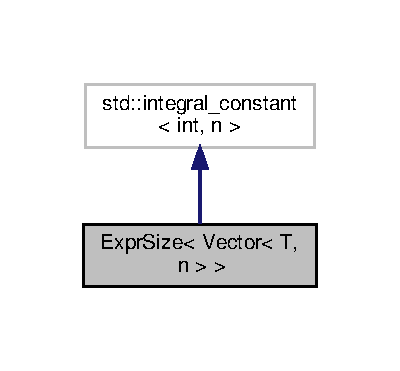
\includegraphics[width=192pt]{classExprSize_3_01Vector_3_01T_00_01n_01_4_01_4__coll__graph}
\end{center}
\end{figure}


The documentation for this class was generated from the following file\+:\begin{DoxyCompactItemize}
\item 
src/vector\+\_\+traits.\+hpp\end{DoxyCompactItemize}

\hypertarget{classMemoryMappedFile}{}\section{Memory\+Mapped\+File Class Reference}
\label{classMemoryMappedFile}\index{Memory\+Mapped\+File@{Memory\+Mapped\+File}}
\subsection*{Public Member Functions}
\begin{DoxyCompactItemize}
\item 
\mbox{\Hypertarget{classMemoryMappedFile_a5ce10934f39355d75803f5674ce92744}\label{classMemoryMappedFile_a5ce10934f39355d75803f5674ce92744}} 
{\bfseries Memory\+Mapped\+File} (const std\+::string \&filename)
\item 
\mbox{\Hypertarget{classMemoryMappedFile_a21c8639f9f40285173a33253c046ff88}\label{classMemoryMappedFile_a21c8639f9f40285173a33253c046ff88}} 
const char $\ast$ {\bfseries begin} ()
\item 
\mbox{\Hypertarget{classMemoryMappedFile_ac1b88239d2ab5d3d70c09d9bca1493c5}\label{classMemoryMappedFile_ac1b88239d2ab5d3d70c09d9bca1493c5}} 
const char $\ast$ {\bfseries end} ()
\item 
\mbox{\Hypertarget{classMemoryMappedFile_adb5dd54a4c6770722d2387775637a52c}\label{classMemoryMappedFile_adb5dd54a4c6770722d2387775637a52c}} 
int {\bfseries size} ()
\end{DoxyCompactItemize}


The documentation for this class was generated from the following file\+:\begin{DoxyCompactItemize}
\item 
src/file\+\_\+io.\+cpp\end{DoxyCompactItemize}

\hypertarget{structparseChunk}{}\section{parse\+Chunk Struct Reference}
\label{structparseChunk}\index{parse\+Chunk@{parse\+Chunk}}


Collaboration diagram for parse\+Chunk\+:
\nopagebreak
\begin{figure}[H]
\begin{center}
\leavevmode
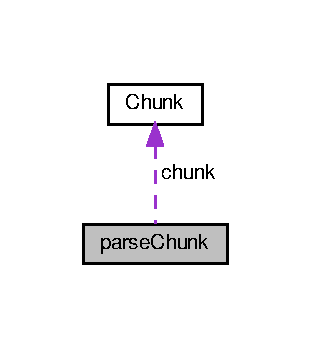
\includegraphics[width=149pt]{structparseChunk__coll__graph}
\end{center}
\end{figure}
\subsection*{Public Member Functions}
\begin{DoxyCompactItemize}
\item 
\mbox{\Hypertarget{structparseChunk_a5aec7c42eb0c0f9fdaa77b879a378019}\label{structparseChunk_a5aec7c42eb0c0f9fdaa77b879a378019}} 
void {\bfseries operator()} ()
\end{DoxyCompactItemize}
\subsection*{Public Attributes}
\begin{DoxyCompactItemize}
\item 
\mbox{\Hypertarget{structparseChunk_ab6b37da3ce4329fff11e7d8b59fb757e}\label{structparseChunk_ab6b37da3ce4329fff11e7d8b59fb757e}} 
\hyperlink{structChunk}{Chunk} {\bfseries chunk}
\item 
\mbox{\Hypertarget{structparseChunk_a5ff5c249a458d01403c0c5b47bb34075}\label{structparseChunk_a5ff5c249a458d01403c0c5b47bb34075}} 
std\+::vector$<$ \hyperlink{structVector}{Vector4f} $>$ \& {\bfseries points}
\item 
\mbox{\Hypertarget{structparseChunk_ac93f102703e2e73a594d23a4dcc19d06}\label{structparseChunk_ac93f102703e2e73a594d23a4dcc19d06}} 
std\+::mutex \& {\bfseries mutex}
\end{DoxyCompactItemize}


The documentation for this struct was generated from the following file\+:\begin{DoxyCompactItemize}
\item 
src/file\+\_\+io.\+cpp\end{DoxyCompactItemize}

\hypertarget{structVector}{}\section{Vector$<$ T, n $>$ Struct Template Reference}
\label{structVector}\index{Vector$<$ T, n $>$@{Vector$<$ T, n $>$}}
\subsection*{Public Member Functions}
\begin{DoxyCompactItemize}
\item 
\mbox{\Hypertarget{structVector_a689be1cfe09cca8fcacec8a5a494fd90}\label{structVector_a689be1cfe09cca8fcacec8a5a494fd90}} 
{\footnotesize template$<$typename ... Ts$>$ }\\constexpr {\bfseries Vector} (Ts ... ts)
\item 
\mbox{\Hypertarget{structVector_ac042df1b1796d2f74fa1b57e678b5cbe}\label{structVector_ac042df1b1796d2f74fa1b57e678b5cbe}} 
constexpr T {\bfseries operator\mbox{[}$\,$\mbox{]}} (const int index) const noexcept
\item 
\mbox{\Hypertarget{structVector_aabe366c7f34fbd7aed51cb1b89e10277}\label{structVector_aabe366c7f34fbd7aed51cb1b89e10277}} 
constexpr T \& {\bfseries operator\mbox{[}$\,$\mbox{]}} (const int index) noexcept
\item 
\mbox{\Hypertarget{structVector_afe385496cc3cc581b050c7e6bcd6296c}\label{structVector_afe385496cc3cc581b050c7e6bcd6296c}} 
constexpr int {\bfseries size} () const noexcept
\item 
\mbox{\Hypertarget{structVector_a93b4267e50ed2889478d9340d2bed3ca}\label{structVector_a93b4267e50ed2889478d9340d2bed3ca}} 
constexpr T {\bfseries norm} () const noexcept
\end{DoxyCompactItemize}


The documentation for this struct was generated from the following file\+:\begin{DoxyCompactItemize}
\item 
src/vector.\+hpp\end{DoxyCompactItemize}

%--- End generated contents ---

% Index
\backmatter
\newpage
\phantomsection
\clearemptydoublepage
\addcontentsline{toc}{chapter}{Index}
\printindex

\end{document}
